%Preamble
\documentclass[12pt]{article}
\usepackage{fancyhdr}
\usepackage{extramarks}
\usepackage{amsmath}
\usepackage{amssymb}
\usepackage{amsthm}
\usepackage{amsrefs}
\usepackage{amsfonts}
\usepackage{mathrsfs}
\usepackage{mathtools}
\usepackage[mathcal]{eucal} %% changes meaning of \mathcal
\usepackage{enumerate}
\usepackage[shortlabels]{enumitem}
\usepackage{verbatim} %% includes comment environment
\usepackage{hyperref}
\usepackage[capitalize]{cleveref}
\crefformat{equation}{~(#2#1#3)}
\usepackage{caption, subcaption}
\usepackage{graphicx}
\usepackage{fullpage} %%smaller margins
\usepackage[all,arc]{xy}
\usepackage{mathrsfs}

\hypersetup{
    linktoc=all,     % set to all if you want both sections and subsections linked
}

\topmargin=-0.45in
\evensidemargin=0in
\oddsidemargin=0in
\textwidth=6.5in
\textheight=9.0in
\headsep=0.25in
\setlength{\headheight}{16pt}

\linespread{1.0}

\pagestyle{fancy}
\lhead{\Name}
\chead{\hwClass: \hwTitle}
\rhead{\hwDueDate}
\lfoot{\lastxmark}
\cfoot{\thepage}

\renewcommand\headrulewidth{0.4pt}
\renewcommand\footrulewidth{0.4pt}

\setlength\parindent{0pt}

%% Title Info
\newcommand{\hwTitle}{HW \# 6}
\newcommand{\hwDueDate}{March 5, 2021}
\newcommand{\hwClass}{AMATH 568}
\newcommand{\hwClassTime}{}
\newcommand{\hwClassInstructor}{}
\newcommand{\Name}{\textbf{Marlin Figgins}}


%% MATH MACROS
\newcommand{\bbF}{\mathbb{F}}
\newcommand{\bbN}{\mathbb{N}}
\newcommand{\bbQ}{\mathbb{Q}}
\newcommand{\bbR}{\mathbb{R}}
\newcommand{\bbZ}{\mathbb{Z}}
\newcommand{\bbC}{\mathbb{C}}
\newcommand{\abs}[1]{ \left| #1 \right| }
\newcommand{\diff}[2]{\frac{d #1}{d #2}}
\newcommand{\infsum}[1]{\sum_{#1}^{\infty}}
\newcommand{\norm}[1]{ \left|\left| #1 \right|\right| }
\newcommand{\eval}[1]{ \left. #1 \right| }
\newcommand{\Expect}[1]{\mathbb{E}\left[#1 \right]}
\newcommand{\Var}[1]{\mathbb{V}\left[#1 \right]}
\renewcommand{\vec}[1]{\mathbf{#1}}

\renewcommand{\phi}{\varphi}
\renewcommand{\emptyset}{\O}

%--------Theorem Environments--------
%theoremstyle{plain} --- defaultx
\newtheorem{thm}{Theorem}[section]
\newtheorem{cor}[thm]{Corollary}
\newtheorem{prop}[thm]{Proposition}
\newtheorem{lem}[thm]{Lemma}
\newtheorem{conj}[thm]{Conjecture}
\newtheorem{quest}[thm]{Question}

\theoremstyle{definition}
\newtheorem{defn}[thm]{Definition}
\newtheorem{defns}[thm]{Definitions}
\newtheorem{con}[thm]{Construction}
\newtheorem{exmp}[thm]{Example}
\newtheorem{exmps}[thm]{Examples}
\newtheorem{notn}[thm]{Notation}
\newtheorem{notns}[thm]{Notations}
\newtheorem{addm}[thm]{Addendum}

% Environments for answers and solutions
\newtheorem{exer}{Exercise}
\newtheorem{sol}{Solution}

\theoremstyle{remark}
\newtheorem{rem}[thm]{Remark}
\newtheorem{rems}[thm]{Remarks}
\newtheorem{warn}[thm]{Warning}
\newtheorem{sch}[thm]{Scholium}

\makeatletter
\let\c@equation\c@thm
\makeatother

\begin{document}

\begin{exer}

Consider the singular equation:
\begin{equation*}
    \epsilon \frac{d^{2} u}{dx^{2}} + (1 + x)^{2} \frac{d u}{d x} + u = 0
\end{equation*}
with $u(0) = u(1) = 1$ and with $0 < \epsilon \ll 1$.
\begin{enumerate}[(a)]
    \item Obtain the leading order uniform solution using the WKB method.
    \item Plot the uniform solution for $\epsilon = 0.01$, $0.05$,  $0.1$,  $0.2$.
\end{enumerate}
\end{exer}

\begin{sol}
    We'll write $u(x)$ using a WKB expansion as follows
    \begin{align*}
        u(x) = \exp\left(  \frac{S_{0}(x) + \epsilon S_{1}(x) + \epsilon^{2} S_{2}(x) + \cdots }{\epsilon} \right).
    \end{align*}
Plugging this expansion into the differential equation of interest, we have
\begin{align*}
    \epsilon \left(  \frac{S_{0x}^{2}(x)}{\epsilon^{2}}+ \frac{2 S_{0x}(x) S_{1x}}{\epsilon}  + \cdots \frac{S_{0xx}}{\epsilon} + \cdots  \right) u(x) +   (1 + x)^{2} \left( \frac{S_{0x}}{\epsilon} + S_{1x}(x) + \cdots    \right) u(x) + u(x) = 0.
\end{align*}
using formula (360) from notes to compute the derivatives of $u$. Collecting powers of $\epsilon$ and removing  $u(x)$ since all terms contain $u$ we have the following hierarchy of equations.
\begin{align*}
    O(\epsilon^{-1}):& \quad S_{0x}^{2}(x) + (1+x)^{2} S_{0x}(x) = 0\\
    O(1):& \quad S_{0xx} + 2 S_{0x}(x) S_{1x}(x) + (1+x)^{2} S_{1x}(x) + 1 = 0.
\end{align*}
This leaves two possible solutions for the $O(\epsilon^{-1})$ term
\begin{align*}
    S_{0x} = 0 &\implies S_{0} = C\\
    S_{0x} = -(1 + x)^{2} &\implies S_{0} = - \frac{(1 + x)^{3}}{3} + C.
\end{align*}
The first case $S_{0x}=0$ reduces the  $O(1)$ equation to
\begin{align*}
    (1+x)^{2} S_{1x}(x) + 1 = 0,
\end{align*}
so that
\begin{align*}
    S_{1x} = - (1 + x)^{-2} \implies S_{1}(x) = \frac{1}{1+x} + C.
\end{align*}
Therefore, our first solution is given by
\begin{align*}
    u(x) = C_{1}\exp\left( \frac{1}{1+x} \right).
\end{align*}
We can now consider the second case which has $O(1)$ equation
\begin{align*}
    2(1+x) - (1 + x)^{2} S_{1x} + 1 = 0
\end{align*}
This has solution
\begin{align*}
    S_{1}(x) = - (1 + x)^{-1} - \ln (1 + x)^{2},
\end{align*}
which when plugged into the expansion gives
\begin{align*}
    u(x) = \frac{C_{2}}{(1+x)^{2}}\exp\left( -\frac{1}{1+x} - \frac{1}{3\epsilon} (1+x)^{3}    \right)
\end{align*}
Our combined uniform solution is then
\begin{align*}
    u(x) = C_{1}\exp\left( \frac{1}{1 + x} \right) + \frac{C_{2}}{(1+x)^{2}}\exp\left( -\frac{1}{1+x} - \frac{1}{3\epsilon} (1+x)^{3} \right).
\end{align*}
We can use the boundary conditions to solve for the constants of interest. We require that
\begin{align*}
    u(0) &= C_{1} e + C_{2} e^{-1} \exp\left(-\frac{1}{3\epsilon}  \right) = 1\\
    u(1) &= C_{1} e^{\frac{1}{2}} + \frac{C_{2}}{4} e^{-\frac{1}{2}}\exp\left( - \frac{8}{3 \epsilon} \right) = 1.
\end{align*}
Starting with the first equation, we write that
\begin{align*}
C_{2} = F e^{1 + \frac{1}{3\epsilon}},
\end{align*}
which allows us to simplfy so that
\begin{align*}
    1  &= C_{1} e + F \\
    1 &= C_{1} e^{-\frac{1}{2}} + \frac{F}{4} \exp\left(\frac{1}{2} - \frac{7}{3} \epsilon\right).
\end{align*}
Noticing that $\exp\left(\frac{1}{2} - \frac{7}{3} \epsilon\right)$ is appoximately 0 in the small $\epsilon$ limit tells us that
 \begin{align*}
     C_{1} &= e^{-\frac{1}{2}} \\
     C_{2} &= (1 - e^{\frac{1}{2}})  e^{1 + \frac{1}{3\epsilon}}.
\end{align*}
This gives solution
\begin{align*}
    u(x) = \exp\left( \frac{1}{1 + x} - \frac{1}{2} \right) 
    + \frac{1 - e^{1 / 2}}{(1+x)^{2}} \exp\left( -\frac{1}{1+x} + 1 - \frac{1}{3\epsilon} \left[(1+x)^{3} - 1 \right] \right).
\end{align*}

\newpage

\begin{figure}[ht]
    \centering
    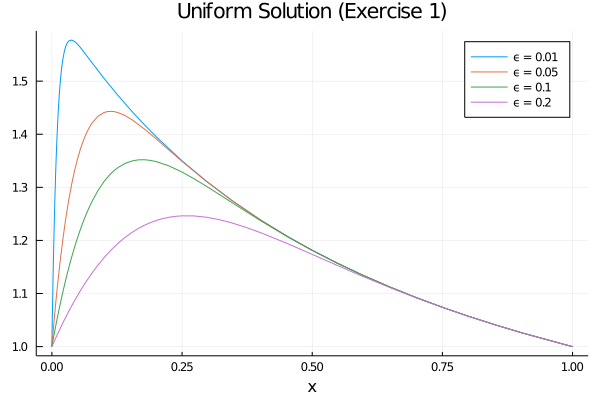
\includegraphics[width=0.8\linewidth]{figs/hw-6-exer-1.png}
    \caption{Uniform solution for various $\epsilon$}%
    \label{fig:figs/hw-6-exer-1}
\end{figure}
\end{sol}
\end{document}
